% 【拆分生成】 questions.tex —— 2017 年·全国Ⅰ卷·理科 · 题目内容片段（无答案）
% 【拆分生成】 由 tools/split_project.py 自合并书 papers/2017_g1_li.tex 包裹 question 环境生成，勿手改
% 由 tools/md2tex.py 自 2017_数学真题_理_试题.md 生成，勿手改（改源 MD 后重跑）


\begin{gknotice}
\textbf{ 卷种提示}：本卷为文理分科时代的旧结构，含\textbf{现已取消}的选做题（第 22/23 题）与\textbf{已删除}的三视图（第 7 题）、程序框图（第 8 题）考点。适合\textbf{按知识点抽题}，不适合整套限时模拟。

\textbf{适用省份}：河南、河北、山西、江西、湖北、湖南、广东、安徽、福建、山东
\end{gknotice}

\par\medskip

\gkpart{一、选择题}

\begin{gktip}
本题共 12 小题，每小题 5 分，共 60 分。
\end{gktip}

\begin{question}
\gkti{1}已知集合 $A=\{x\mid x<1\}$，$B=\left\{x\mid3^{x}<1\right\}$，则（　　）

\begin{gkopts}(2)
\task A．$A\cap B=\{x\mid x<0\}$
\task B．$A\cup B=\mathbf R$
\task C．$A\cup B=\{x\mid x>1\}$
\task D．$A\cap B=\varnothing$
\end{gkopts}

\end{question}
\begin{question}
\gkti{2}如图，正方形 $ABCD$ 内的图形来自中国古代的太极图，正方形内切圆中的黑色部分和白色部分关于正方形的中心成中心对称。在正方形内随机取一点，则此点取自黑色部分的概率是（　　）

\begin{center}% 2017 全国Ⅰ卷 理2/文4：正方形内的太极图（黑白关于中心成中心对称）
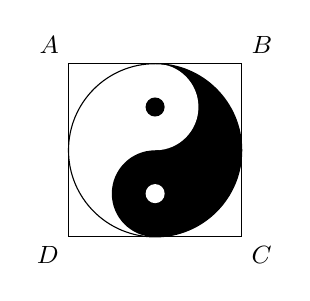
\begin{tikzpicture}[scale=1.1, font=\small]
  % 正方形 ABCD（A 左上、B 右上、C 右下、D 左下），边长 2，内切圆半径 1
  \draw (-1,-1) rectangle (1,1);
  \node[above left]  at (-1, 1) {$A$};
  \node[above right] at ( 1, 1) {$B$};
  \node[below right] at ( 1,-1) {$C$};
  \node[below left]  at (-1,-1) {$D$};
  \begin{scope}
    \clip (0,0) circle (1);
    % 右半黑
    \fill[black] (0,1) arc (90:-90:1) -- cycle;
    % 上小圆白、下小圆黑，构成 S 形分界
    \fill[white] (0,0.5) circle (0.5);
    \fill[black] (0,-0.5) circle (0.5);
    % 鱼眼
    \fill[black] (0,0.5) circle (0.11);
    \fill[white] (0,-0.5) circle (0.11);
  \end{scope}
  \draw (0,0) circle (1);
\end{tikzpicture}
\end{center}

\begin{gkopts}(4)
\task A．$\dfrac14$
\task B．$\dfrac\pi8$
\task C．$\dfrac12$
\task D．$\dfrac\pi4$
\end{gkopts}

\end{question}
\begin{question}
\gkti{3}设有下面四个命题：

  $p_1$：若复数 $z$ 满足 $\dfrac1z\in\mathbf R$，则 $z\in\mathbf R$；

  $p_2$：若复数 $z$ 满足 $z^{2}\in\mathbf R$，则 $z\in\mathbf R$；

  $p_3$：若复数 $z_1$，$z_2$ 满足 $z_1z_2\in\mathbf R$，则 $z_1=\overline{z_2}$；

  $p_4$：若复数 $z\in\mathbf R$，则 $\bar z\in\mathbf R$。

其中的真命题为（　　）

\begin{gkopts}(4)
\task A．$p_1$，$p_3$
\task B．$p_1$，$p_4$
\task C．$p_2$，$p_3$
\task D．$p_2$，$p_4$
\end{gkopts}

\end{question}
\begin{question}
\gkti{4}记 $S_n$ 为等差数列 $\left\{a_n\right\}$ 的前 $n$ 项和。若 $a_4+a_5=24$，$S_6=48$，则 $\left\{a_n\right\}$ 的公差为（　　）

\begin{gkopts}(4)
\task A．$1$
\task B．$2$
\task C．$4$
\task D．$8$
\end{gkopts}

\end{question}
\begin{question}
\gkti{5}函数 $f(x)$ 在 $(-\infty,+\infty)$ 单调递减，且为奇函数。若 $f(1)=-1$，则满足 $-1\le f(x-2)\le1$ 的 $x$ 的取值范围是（　　）

\begin{gkopts}(4)
\task A．$[-2,2]$
\task B．$[-1,1]$
\task C．$[0,4]$
\task D．$[1,3]$
\end{gkopts}

\end{question}
\begin{question}
\gkti{6}$\left(1+\dfrac1{x^{2}}\right)(1+x)^{6}$ 展开式中 $x^{2}$ 的系数为（　　）

\begin{gkopts}(4)
\task A．$15$
\task B．$20$
\task C．$30$
\task D．$35$
\end{gkopts}

\end{question}
\begin{question}
\gkti{7}某多面体的三视图如图所示，其中正视图和左视图都由正方形和等腰直角三角形组成，正方形的边长为 $2$，俯视图为等腰直角三角形。该多面体的各个面中有若干个是梯形，这些梯形的面积之和为（　　）

\begin{center}% 2017 全国Ⅰ卷 理7：多面体三视图
% 正视图/左视图 = 边长 2 的正方形上叠等腰直角三角形；俯视图 = 等腰直角三角形
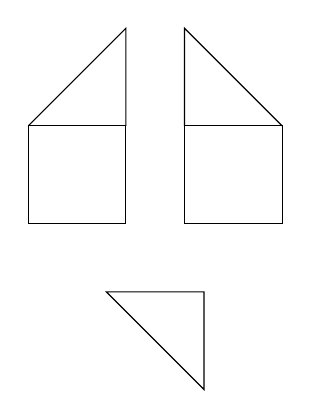
\begin{tikzpicture}[scale=0.62, font=\small]
  % 正视图（三角形直角边在右）
  \begin{scope}
    \draw (0,0) rectangle (2,2);
    \draw (0,2) -- (2,4) -- (2,2);
  \end{scope}
  % 左视图（三角形直角边在左）
  \begin{scope}[xshift=3.2cm]
    \draw (0,0) rectangle (2,2);
    \draw (0,2) -- (0,4) -- (2,2);
  \end{scope}
  % 俯视图（等腰直角三角形，直角边 2）
  \begin{scope}[yshift=-3.4cm, xshift=1.6cm]
    \draw (0,2) -- (2,2) -- (2,0) -- cycle;
  \end{scope}
\end{tikzpicture}
\end{center}

\begin{gkopts}(4)
\task A．$10$
\task B．$12$
\task C．$14$
\task D．$16$
\end{gkopts}

\begin{gktip}
\textbf{注}：三视图在现行新课标中已删除。
\end{gktip}

\end{question}
\begin{question}
\gkti{8}如图程序框图是为了求出满足 $3^{n}-2^{n}>1000$ 的最小偶数 $n$，那么在 $\Diamond$ 和 $\square$ 两个空白框中，可以分别填入（　　）

\begin{center}% 2017 全国Ⅰ卷 理8/文10：求满足 3^n-2^n>1000 的最小偶数 n 的程序框图
% 两个空白框（菱形与左侧矩形）是题目要求填入的位置，故留白
\begin{tikzpicture}[font=\small, >=Stealth, node distance=8mm,
  box/.style={draw, minimum height=1.9em, inner xsep=7pt},
  term/.style={draw, rounded corners=7pt, minimum height=1.9em, inner xsep=9pt},
  io/.style={draw, trapezium, trapezium left angle=70, trapezium right angle=110,
             minimum height=1.9em, inner xsep=2pt},
  dec/.style={draw, diamond, aspect=2.4, inner sep=1.5pt}]
  \node[term] (start) {开始};
  \node[io, below=of start] (in) {输入 $n=0$};
  \coordinate[below=5mm of in] (merge);
  \node[box, below=2mm of merge] (calc) {$A=3^{n}-2^{n}$};
  \node[dec, below=of calc] (cond) {\phantom{$A\le1000$}};
  \node[box, left=12mm of calc, minimum width=5.2em] (blank) {\phantom{$n=n+2$}};
  \node[io, below=of cond] (out) {输出 $n$};
  \node[term, below=of out] (end) {结束};
  \draw[->] (start) -- (in);
  \draw[->] (in) -- (calc);
  \draw[->] (calc) -- (cond);
  \draw[->] (cond) -- node[right]{否} (out);
  \draw[->] (out) -- (end);
  \draw[->] (cond) -| node[below, pos=0.18]{是} (blank);
  \draw[->] (blank) |- (merge);
\end{tikzpicture}
\end{center}

\begin{gkopts}(2)
\task A．$A>1000$ 和 $n=n+1$
\task B．$A>1000$ 和 $n=n+2$
\task C．$A\le1000$ 和 $n=n+1$
\task D．$A\le1000$ 和 $n=n+2$
\end{gkopts}

\begin{gktip}
\textbf{注}：程序框图（算法初步）在现行新课标中已删除。
\end{gktip}

\end{question}
\begin{question}
\gkti{9}已知曲线 $C_1:y=\cos x$，$C_2:y=\sin\left(2x+\dfrac{2\pi}3\right)$，则下面结论正确的是（　　）

\begin{gkopts}(1)
\task A．把 $C_1$ 上各点的横坐标伸长到原来的 $2$ 倍，纵坐标不变，再把得到的曲线向右平移 $\dfrac\pi6$ 个单位长度，得到曲线 $C_2$
\task B．把 $C_1$ 上各点的横坐标伸长到原来的 $2$ 倍，纵坐标不变，再把得到的曲线向左平移 $\dfrac\pi{12}$ 个单位长度，得到曲线 $C_2$
\task C．把 $C_1$ 上各点的横坐标缩短到原来的 $\dfrac12$ 倍，纵坐标不变，再把得到的曲线向右平移 $\dfrac\pi6$ 个单位长度，得到曲线 $C_2$
\task D．把 $C_1$ 上各点的横坐标缩短到原来的 $\dfrac12$ 倍，纵坐标不变，再把得到的曲线向左平移 $\dfrac\pi{12}$ 个单位长度，得到曲线 $C_2$
\end{gkopts}

\end{question}
\begin{question}
\gkti{10}已知 $F$ 为抛物线 $C:y^{2}=4x$ 的焦点，过 $F$ 作两条互相垂直的直线 $l_1$，$l_2$，直线 $l_1$ 与 $C$ 交于 $A$，$B$ 两点，直线 $l_2$ 与 $C$ 交于 $D$，$E$ 两点，则 $|AB|+|DE|$ 的最小值为（　　）

\begin{gkopts}(4)
\task A．$16$
\task B．$14$
\task C．$12$
\task D．$10$
\end{gkopts}

\end{question}
\begin{question}
\gkti{11}设 $x$，$y$，$z$ 为正数，且 $2^{x}=3^{y}=5^{z}$，则（　　）

\begin{gkopts}(4)
\task A．$2x<3y<5z$
\task B．$5z<2x<3y$
\task C．$3y<5z<2x$
\task D．$3y<2x<5z$
\end{gkopts}

\end{question}
\begin{question}
\gkti{12}几位大学生响应国家的创业号召，开发了一款应用软件。为激发大家学习数学的兴趣，他们推出了"解数学题获取软件激活码"的活动。这款软件的激活码为下面数学问题的答案：已知数列 $1$，$1$，$2$，$1$，$2$，$4$，$1$，$2$，$4$，$8$，$1$，$2$，$4$，$8$，$16$，$\cdots$，其中第一项是 $2^{0}$，接下来的两项是 $2^{0}$，$2^{1}$，再接下来的三项是 $2^{0}$，$2^{1}$，$2^{2}$，依此类推。求满足如下条件的最小整数 $N$：$N>100$ 且该数列的前 $N$ 项和为 $2$ 的整数幂。那么该款软件的激活码是（　　）

\begin{gkopts}(4)
\task A．$440$
\task B．$330$
\task C．$220$
\task D．$110$
\end{gkopts}

\par\medskip

\end{question}
\gkpart{二、填空题}

\begin{gktip}
本题共 4 小题，每小题 5 分，共 20 分。
\end{gktip}

\begin{question}
\gkti{13}已知向量 $\boldsymbol a$，$\boldsymbol b$ 的夹角为 $60^\circ$，$|\boldsymbol a|=2$，$|\boldsymbol b|=1$，则 $|\boldsymbol a+2\boldsymbol b|=$ \gkblank{}．

\end{question}
\begin{question}
\gkti{14}设 $x$，$y$ 满足约束条件 $\begin{cases}x+2y\le1\\ 2x+y\ge-1\\ x-y\le0\end{cases}$，则 $z=3x-2y$ 的最小值为 \gkblank{}．

\end{question}
\begin{question}
\gkti{15}已知双曲线 $C:\dfrac{x^{2}}{a^{2}}-\dfrac{y^{2}}{b^{2}}=1\ (a>0,\ b>0)$ 的右顶点为 $A$，以 $A$ 为圆心、$b$ 为半径作圆 $A$，圆 $A$ 与双曲线 $C$ 的一条渐近线交于 $M$，$N$ 两点。若 $\angle MAN=60^\circ$，则 $C$ 的离心率为 \gkblank{}．

\end{question}
\begin{question}
\gkti{16}如图，圆形纸片的圆心为 $O$，半径为 $5\ \mathrm{cm}$，该纸片上的等边三角形 $ABC$ 的中心为 $O$。$D$，$E$，$F$ 为圆 $O$ 上的点，$\triangle DBC$，$\triangle ECA$，$\triangle FAB$ 分别是以 $BC$，$CA$，$AB$ 为底边的等腰三角形。沿虚线剪开后，分别以 $BC$，$CA$，$AB$ 为折痕折起 $\triangle DBC$，$\triangle ECA$，$\triangle FAB$，使得 $D$，$E$，$F$ 重合，得到三棱锥。当 $\triangle ABC$ 的边长变化时，所得三棱锥体积（单位：$\mathrm{cm}^{3}$）的最大值为 \gkblank{}．

\begin{center}% 2017 全国Ⅰ卷 理16：圆形纸片（半径 5）与内接等边三角形 ABC，
% D、E、F 为圆上的点，分别与 BC、CA、AB 构成待折起的等腰三角形
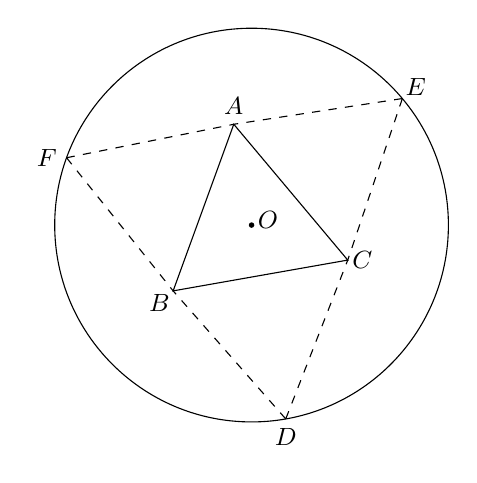
\begin{tikzpicture}[scale=1.0, font=\small]
  \def\R{2.5}      % 圆半径（示意比例）
  \def\r{1.3}      % 三角形中心到顶点距离
  \draw (0,0) circle (\R);
  \coordinate (A) at (100:\r);
  \coordinate (B) at (220:\r);
  \coordinate (C) at (-20:\r);
  \coordinate (D) at (280:\R);
  \coordinate (E) at (40:\R);
  \coordinate (F) at (160:\R);
  \draw (A) -- (B) -- (C) -- cycle;
  \draw[dashed] (D) -- (B) (D) -- (C);
  \draw[dashed] (E) -- (C) (E) -- (A);
  \draw[dashed] (F) -- (A) (F) -- (B);
  \fill (0,0) circle (1pt);
  \node[right, inner sep=1.5pt] at (0.02,0.06) {$O$};
  \node[above] at (A) {$A$};
  \node[below left, inner sep=1pt] at (B) {$B$};
  \node[right, inner sep=1.5pt] at (C) {$C$};
  \node[below] at (D) {$D$};
  \node[above right, inner sep=1pt] at (E) {$E$};
  \node[left] at (F) {$F$};
\end{tikzpicture}
\end{center}

\par\medskip

\end{question}
\gkpart{三、解答题}

\begin{gktip}
共 70 分。第 17～21 题为必考题，第 22、23 题为选考题。
\end{gktip}

\gksubpart{（一）必考题：共 60 分}

\begin{question}
\gkti{17}\textbf{（12 分）} $\triangle ABC$ 的内角 $A$，$B$，$C$ 的对边分别为 $a$，$b$，$c$，已知 $\triangle ABC$ 的面积为 $\dfrac{a^{2}}{3\sin A}$。

  (1) 求 $\sin B\sin C$；

  (2) 若 $6\cos B\cos C=1$，$a=3$，求 $\triangle ABC$ 的周长。

\end{question}
\begin{question}
\gkti{18}\textbf{（12 分）} 如图，在四棱锥 $P\text{-}ABCD$ 中，$AB\parallel CD$，且 $\angle BAP=\angle CDP=90^\circ$。

\begin{center}% 2017 全国Ⅰ卷 理18/文18：四棱锥 P-ABCD（AB∥CD，∠BAP=∠CDP=90°）
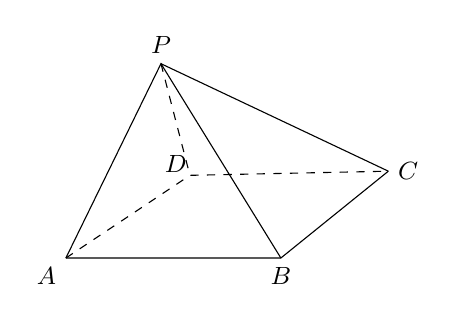
\begin{tikzpicture}[scale=1.05, font=\small]
  \coordinate (P) at (1.15,2.35);
  \coordinate (A) at (0,0);
  \coordinate (B) at (2.6,0);
  \coordinate (C) at (3.9,1.05);
  \coordinate (D) at (1.5,1.0);
  \draw (A) -- (B) -- (C);
  \draw (A) -- (P) -- (B);
  \draw (P) -- (C);
  \draw[dashed] (A) -- (D) -- (C);
  \draw[dashed] (P) -- (D);
  \node[above] at (P) {$P$};
  \node[below left] at (A) {$A$};
  \node[below] at (B) {$B$};
  \node[right] at (C) {$C$};
  \node[above left, inner sep=1pt] at (D) {$D$};
\end{tikzpicture}
\end{center}

  (1) 证明：平面 $PAB\perp$ 平面 $PAD$；

  (2) 若 $PA=PD=AB=DC$，$\angle APD=90^\circ$，求二面角 $A\text{-}PB\text{-}C$ 的余弦值。

\end{question}
\begin{question}
\gkti{19}\textbf{（12 分）} 为了监控某种零件的一条生产线的生产过程，检验员每天从该生产线上随机抽取 $16$ 个零件，并测量其尺寸（单位：$\mathrm{cm}$）。根据长期生产经验，可以认为这条生产线正常状态下生产的零件的尺寸服从正态分布 $N\left(\mu,\sigma^{2}\right)$。

  (1) 假设生产状态正常，记 $X$ 表示一天内抽取的 $16$ 个零件中其尺寸在 $(\mu-3\sigma,\ \mu+3\sigma)$ 之外的零件数，求 $P(X\ge1)$ 及 $X$ 的数学期望；

  (2) 一天内抽检零件中，如果出现了尺寸在 $(\mu-3\sigma,\ \mu+3\sigma)$ 之外的零件，就认为这条生产线在这一天的生产过程可能出现了异常情况，需对当天的生产过程进行检查。

  　① 试说明上述监控生产过程方法的合理性；

  　② 下面是检验员在一天内抽取的 $16$ 个零件的尺寸：

\begin{center}
\begin{tabular}{cccccccc}
\toprule
$9.95$ & $10.12$ & $9.96$ & $9.96$ & $10.01$ & $9.92$ & $9.98$ & $10.04$ \\
\midrule
$10.26$ & $9.91$ & $10.13$ & $10.02$ & $9.22$ & $10.04$ & $10.05$ & $9.95$ \\
\bottomrule
\end{tabular}
\end{center}

  经计算得 $\bar x=\dfrac1{16}\sum\limits_{i=1}^{16}x_i=9.97$，$s=\sqrt{\dfrac1{16}\sum\limits_{i=1}^{16}\left(x_i-\bar x\right)^{2}}=\sqrt{\dfrac1{16}\left(\sum\limits_{i=1}^{16}x_i^{2}-16\bar x^{2}\right)}\approx0.212$，其中 $x_i$ 为抽取的第 $i$ 个零件的尺寸，$i=1,2,\cdots,16$。

  用样本平均数 $\bar x$ 作为 $\mu$ 的估计值 $\hat\mu$，用样本标准差 $s$ 作为 $\sigma$ 的估计值 $\hat\sigma$，利用估计值判断是否需对当天的生产过程进行检查？剔除 $\left(\hat\mu-3\hat\sigma,\ \hat\mu+3\hat\sigma\right)$ 之外的数据，用剩下的数据估计 $\mu$ 和 $\sigma$（精确到 $0.01$）。

  附：若随机变量 $Z$ 服从正态分布 $N\left(\mu,\sigma^{2}\right)$，则 $P(\mu-3\sigma<Z<\mu+3\sigma)=0.9974$，$0.9974^{16}\approx0.9592$，$\sqrt{0.008}\approx0.09$。

\end{question}
\begin{question}
\gkti{20}\textbf{（12 分）} 已知椭圆 $C:\dfrac{x^{2}}{a^{2}}+\dfrac{y^{2}}{b^{2}}=1\ (a>b>0)$，四点 $P_1(1,1)$，$P_2(0,1)$，$P_3\left(-1,\dfrac{\sqrt3}2\right)$，$P_4\left(1,\dfrac{\sqrt3}2\right)$ 中恰有三点在椭圆 $C$ 上。

  (1) 求 $C$ 的方程；

  (2) 设直线 $l$ 不经过 $P_2$ 点且与 $C$ 相交于 $A$，$B$ 两点。若直线 $P_2A$ 与直线 $P_2B$ 的斜率的和为 $-1$，证明：$l$ 过定点。

\end{question}
\begin{question}
\gkti{21}\textbf{（12 分）} 已知函数 $f(x)=a\mathrm e^{2x}+(a-2)\mathrm e^{x}-x$。

  (1) 讨论 $f(x)$ 的单调性；

  (2) 若 $f(x)$ 有两个零点，求 $a$ 的取值范围。

\par\medskip

\end{question}
\gksubpart{（二）选考题：共 10 分，第 22、23 题任选一题作答}

\begin{gktip}
\textbf{ 现行考纲已取消选做题}，以下两题仅作历史资料保留。
\end{gktip}

\begin{question}
\gkti{22}\textbf{（10 分）〔选修 4-4：坐标系与参数方程〕} （\textbf{已取消}）

在直角坐标系 $xOy$ 中，曲线 $C$ 的参数方程为 $\begin{cases}x=3\cos\theta\\ y=\sin\theta\end{cases}$（$\theta$ 为参数），直线 $l$ 的参数方程为 $\begin{cases}x=a+4t\\ y=1-t\end{cases}$（$t$ 为参数）。

  (1) 若 $a=-1$，求 $C$ 与 $l$ 的交点坐标；

  (2) 若 $C$ 上的点到 $l$ 距离的最大值为 $\sqrt{17}$，求 $a$。

\end{question}
\begin{question}
\gkti{23}\textbf{（10 分）〔选修 4-5：不等式选讲〕} （\textbf{已取消}）

已知函数 $f(x)=-x^{2}+ax+4$，$g(x)=|x+1|+|x-1|$。

  (1) 当 $a=1$ 时，求不等式 $f(x)\ge g(x)$ 的解集；

  (2) 若不等式 $f(x)\ge g(x)$ 的解集包含 $[-1,1]$，求 $a$ 的取值范围。

\par\medskip


\end{question}